\documentclass[../AnalisiDeiRequisiti_v4.0.0.tex]{subfiles}
\begin{document}

\section{Casi d'uso}
Di seguito verranno elencati i casi d'uso ricavati dall'analisi del capitolato C2 e dalle riunioni fatte con \prop.\\
Ogni caso d'uso viene identificato dalla seguente dicitura:
\begin{equation*}
	UC[codice]
\end{equation*}
Dove codice indica il codice univoco con cui verrà indicato ogni caso d'uso.

\subsection{UCG Utente} 
\label{sssec:UCG_Utente}
\begin{figure}[!h]
	\centering
	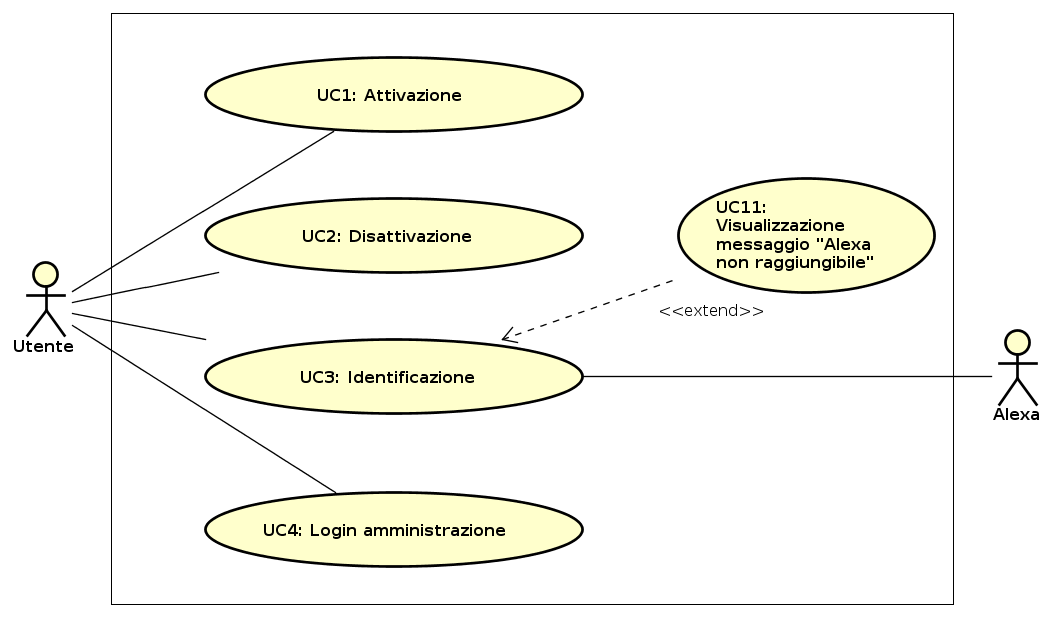
\includegraphics[width=\textwidth]{UseCases/UCG_Utente/UCG_Utente.png}
	\caption{Caso d'uso generale Utente}
\end{figure}
\begin{itemize} 
\item \textbf{Attori}: Utente, Alexa.
\item \textbf{Descrizione}: l'utente può attivare il sistema, disattivarlo, identificarsi, ed un utente amministratore può effettuare il login presso l'area amministrativa.
\item \textbf{Scenario principale}: l'utente attiva il sistema, lo disattiva, si identifica. Un amministratore effettua il login presso l'area amministrativa.
\end{itemize}
\newpage
\subsection{UCG Ospite} 
\label{sssec:UCG_Ospite}
\begin{figure}[!h]
	\centering
	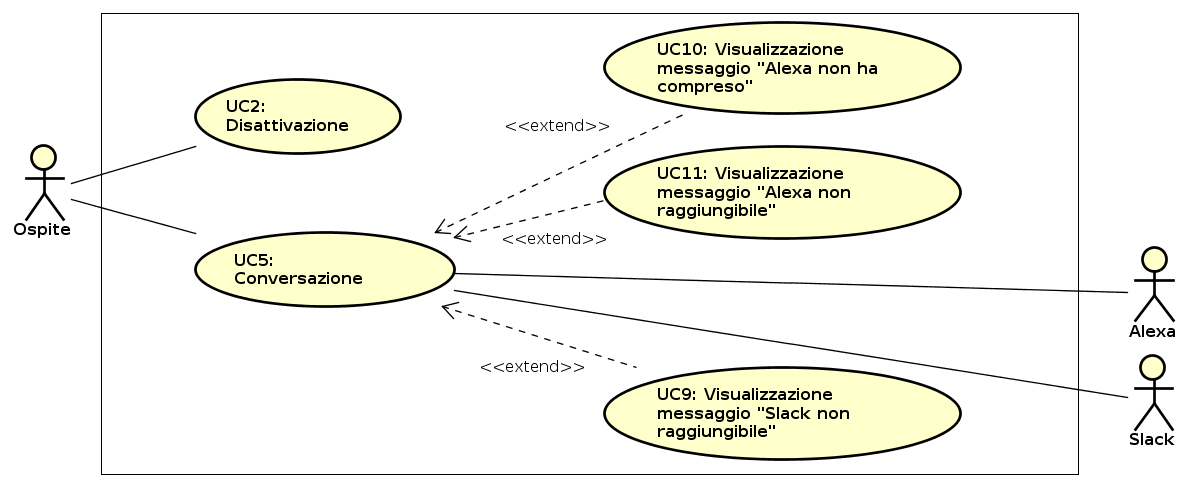
\includegraphics[width=\textwidth]{UseCases/UCG_Ospite/UCG_Ospite.png}
	\caption{Caso d'uso generale Utente}
\end{figure}
\begin{itemize} 
\item \textbf{Attori}: Ospite, Alexa, Slack.
\item \textbf{Descrizione}: un ospite può terminare la sessione attiva e conversare con il sistema tramite una serie di domande e risposte.
\item \textbf{Scenario principale}: l'ospite termina la sessione attiva ed è abilitato a conversare con il sistema.
\end{itemize}
\newpage
\subsection{UCG Amministratore} 
\label{sssec:UCG_Admin} 
\begin{figure}[!h]
	\centering
	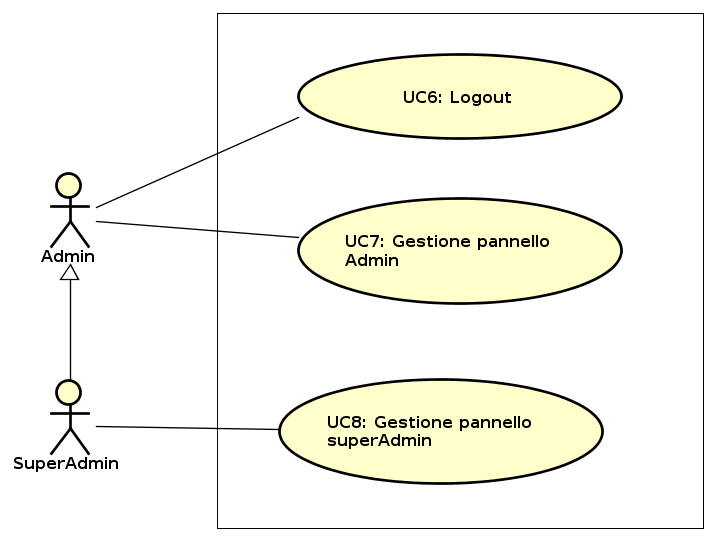
\includegraphics[width=\textwidth]{UseCases/UCG_Amministratore/UCG_Amministratore.png}
	\caption{Caso d'uso generale Amministratore}
\end{figure}
\begin{itemize} 
\item \textbf{Attori}: Admin, SuperAdmin.
\item \textbf{Descrizione}: un amministratore può effettuare il logout dall'area amministrativa oppure utilizzare le funzionalità messe a disposizione dal sistema. Un SuperAdmin può gestire ulteriori funzionalità.
\item \textbf{Scenario principale}: l'amministratore effettua il logout dall'area amministrativa od utilizza le funzionalità messe a disposizione dal sistema. Un SuperAdmin, invece, riesce ad usufruire di ulteriori funzionalità.
\end{itemize}
\newpage
\subsection{UC1 - Attivazione} 
\label{sssec:UC1}
\begin{itemize} 
\item \textbf{Attori}: Utente.
\item \textbf{Descrizione}: l'utente può attivare il sistema;
\item \textbf{Precondizione}: il sistema non è attivo e nessun utente è al momento identificato;
\item \textbf{Postcondizione}: il sistema è attivo e nessun utente è al momento identificato;
\item \textbf{Scenario principale}: l'utente attiva il sistema;
\end{itemize} 
\subsection{UC2 - Disattivazione} 
\label{sssec:UC2}
\begin{figure}[!h]
	\centering
	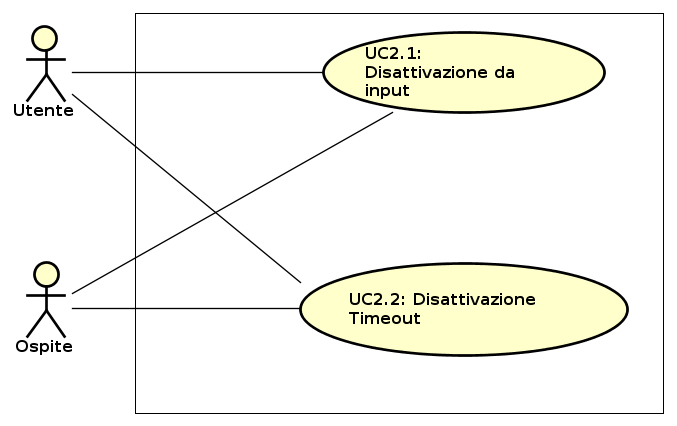
\includegraphics[width=\textwidth]{UseCases/UC2_Disattivazione/UC2_Disattivazione.png}
	\caption{UC2 - Disattivazione}
\end{figure}
\begin{itemize} 
\item \textbf{Attori}: Ospite, Utente.
\item \textbf{Descrizione}: l'utente può disattivare il sistema;
\item \textbf{Precondizione}: il sistema è attivo e un utente o ospite è al momento identificato;
\item \textbf{Postcondizione}: il sistema non è attivo e nessun utente è più identificato;
\item \textbf{Scenario principale}: \begin{enumerate}\item Disattivazione da input (UC2.1);\item Disattivazione per timeout (UC2.2). 
 \end{enumerate}
\end{itemize} 
\subsection{UC2.1 - Disattivazione da input} 
\label{sssec:UC2.1} 
\begin{itemize} 
\item \textbf{Attori}: Ospite, Utente.
\item \textbf{Descrizione}: il sistema può essere disattivato da un utente o un ospite tramite la pressione di un pulsante sullo schermo o un comando vocale in qualsiasi momento;
\item \textbf{Precondizione}: il sistema è correttamente avviato;
\item \textbf{Postcondizione}: il sistema è disattivato e disponibile per un nuovo utente o ospite;
\item \textbf{Scenario principale}: l'utente o l'ospite disattivano il sistema tramite la pressione di un pulsante sullo schermo o di un comando vocale in qualsiasi momento;
\end{itemize} 
\subsection{UC2.2 - Disattivazione per timeout} 
\label{sssec:UC2.2} 
\begin{itemize} 
\item \textbf{Attori}: Ospite, Utente.
\item \textbf{Descrizione}: il sistema può disattivarsi per timeout se non riceve risposta dall'utente o dall'ospite entro un determinato lasso di tempo;
\item \textbf{Precondizione}: il sistema è avviato correttamente e sta attendendo risposta da un utente o ospite;
\item \textbf{Postcondizione}: il sistema è disattivato e disponibile per un nuovo utente o ospite;
\item \textbf{Scenario principale}: l'utente o l'ospite possono disattivare il sistema per timeout se non forniscono una risposta entro un determinato lasso di tempo;
\end{itemize} 
\subsection{UC3 - Identificazione} 
\label{sssec:UC3} 
\begin{figure}[!h]
	\centering
	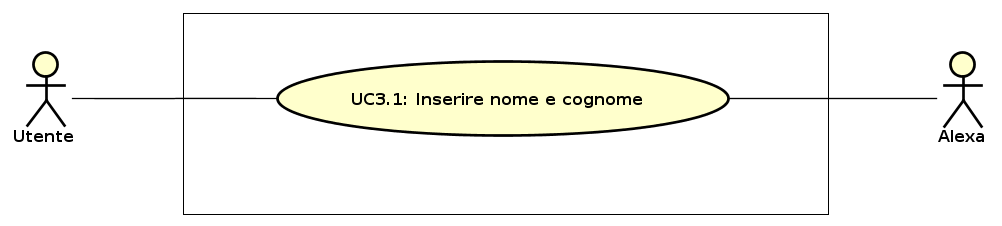
\includegraphics[width=\textwidth]{UseCases/UC3_Identificazione/UC3_Identificazione.png}
	\caption{UC3 - Identificazione}
\end{figure}
\begin{itemize} 
\item \textbf{Attori}: Alexa, Utente.
\item \textbf{Descrizione}: l'utente può identificarsi nel sistema rispondendo alle domande postegli dal sistema;
\item \textbf{Precondizione}: il sistema è attivo e non ha nessun utente identificato;
\item \textbf{Postcondizione}: il sistema è attivo e ha un utente identificato;
\item \textbf{Scenario principale}: \begin{enumerate}\item Inserire nome e cognome (UC3.1). 
 \end{enumerate}
\end{itemize} 
\subsection{UC3.1 - Inserire nome e cognome} 
\label{sssec:UC3.1} 
\begin{itemize} 
\item \textbf{Attori}: Alexa, Utente.
\item \textbf{Descrizione}: l'utente può identificarsi nel sistema inserendo nome e cognome vocalmente o tramite tastiera;
\item \textbf{Precondizione}: Alexa è disponibile e correttamente funzionante. Il sistema non ha nessun utente identificato. Il sistema chiede all'utente di identificarsi con nome e cognome;
\item \textbf{Postcondizione}: il sistema riceve un input dall'utente e procede con l'identificazione dell'utente;
\item \textbf{Scenario principale}: l'utente si identifica nel sistema inserendo nome e cognome vocalmente o tramite tastiera;
\end{itemize} 
\subsection{UC4 - Login amministrazione} 
\label{sssec:UC4} 
\begin{figure}[!h]
	\centering
	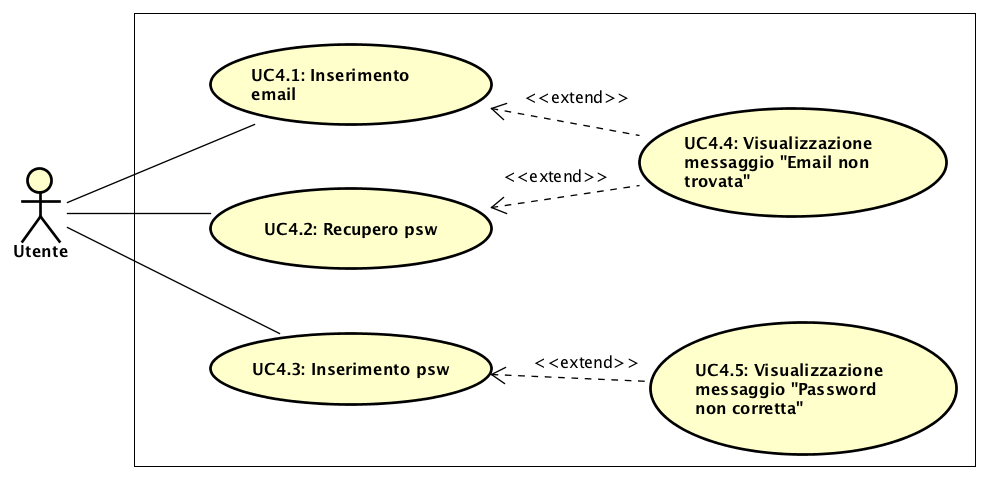
\includegraphics[width=\textwidth]{UseCases/UC4_LoginAmministrazione/UC4_LoginAmministrazione.png}
	\caption{UC4 - Login amministrazione}
\end{figure}
\begin{itemize} 
\item \textbf{Attori}: Utente.
\item \textbf{Descrizione}: un utente amministratore può effettuare il login per la gestione di tutta la console amministrativa;
\item \textbf{Precondizione}: l'utente amministratore non è al momento autenticato nel sistema;
\item \textbf{Postcondizione}: l'utente amministratore è autenticato nel sistema;
\item \textbf{Scenario principale}: \begin{enumerate}\item Inserimento email (UC4.1);\item Recupero password (UC4.2);\item Inserimento password (UC4.3). 
 \end{enumerate}
\item \textbf{Estensioni}:\begin{itemize}\item Visualizzazione messaggio "Email non trovata" (UC4.4).\end{itemize}
\end{itemize} 
\subsection{UC4.1 - Inserimento email} 
\label{sssec:UC4.1} 
\begin{itemize} 
\item \textbf{Attori}: Utente.
\item \textbf{Descrizione}: l'utente amministratore sta effettuando il login e sta inserendo la email;
\item \textbf{Precondizione}: l'utente amministratore non è ancora loggato nel sistema;
\item \textbf{Postcondizione}: l'utente amministratore ha inserito una email;
\item \textbf{Scenario principale}: l'utente amministratore effettua il login ed inserisce la email;
\end{itemize} 
\subsection{UC4.2 - Recupero password} 
\label{sssec:UC4.2} 
\begin{itemize} 
\item \textbf{Attori}: Utente.
\item \textbf{Descrizione}: l'utente amministratore ha dimenticato la password e per recuperarla deve inserire la propria email;
\item \textbf{Precondizione}: l'utente amministratore non è loggato nel sistema;
\item \textbf{Postcondizione}: l'utente amministratore ha inserito la propria email per effettuare il recupero della password;
\item \textbf{Scenario principale}: l'utente amministratore ha dimenticato la password ed inserisce la propria email per recuperarla;
\end{itemize} 
\subsection{UC4.3 - Inserimento password} 
\label{sssec:UC4.3} 
\begin{itemize} 
\item \textbf{Attori}: Utente.
\item \textbf{Descrizione}: l'utente amministratore può inserire una password;
\item \textbf{Precondizione}: l'utente amministratore non è ancora loggato nel sistema;
\item \textbf{Postcondizione}: l'utente amministratore ha inserito una password;
\item \textbf{Scenario principale}: l'utente amministratore inserisce una password;
\item \textbf{Estensioni}:\begin{itemize}\item Visualizzazione messaggio "Password non corretta" (UC4.5).\end{itemize}
\end{itemize} 
\subsection{UC4.5 - Visualizzazione messaggio "Password non corretta"} 
\label{sssec:UC4.5} 
\begin{itemize} 
\item \textbf{Attori}: Utente.
\item \textbf{Descrizione}: il sistema comunica all'amministratore che la password inserita non è corretta, dopo che egli abbia cercato di effettuare il login presso l'area amministrativa;
\item \textbf{Precondizione}: l'utente amministratore ha inserito email e password e cerca di effettuare il login;
\item \textbf{Postcondizione}: l'utente amministratore visualizza un errore di password non corretta;
\item \textbf{Scenario principale}: l'utente amministratore sta cercando di effettuare il login presso l'area amministrativa ma la password inserita non è corretta;
\end{itemize} 
\subsection{UC4.4 - Visualizzazione messaggio "Email non trovata"} 
\label{sssec:UC4.4} 
\begin{itemize} 
\item \textbf{Attori}: Utente.
\item \textbf{Descrizione}: l'utente amministratore sta cercando di effettuare il login presso l'area amministrativa ma nessuna email corrispondente a quella inserita è stata trovata;
\item \textbf{Precondizione}: l'utente amministratore ha inserito email e password e cerca di effettuare il login;
\item \textbf{Postcondizione}: l'utente amministratore visualizza un errore di email non corretta;
\item \textbf{Scenario principale}: l'utente amministratore tenta di effettuare il login presso l'area amministrativa ma è stata trovata nessuna email corrispondente a quella inserita;
\newpage
\end{itemize} 
\subsection{UC5 - Conversazione} 
\label{sssec:UC5}
\begin{figure}[!h]
	\centering
	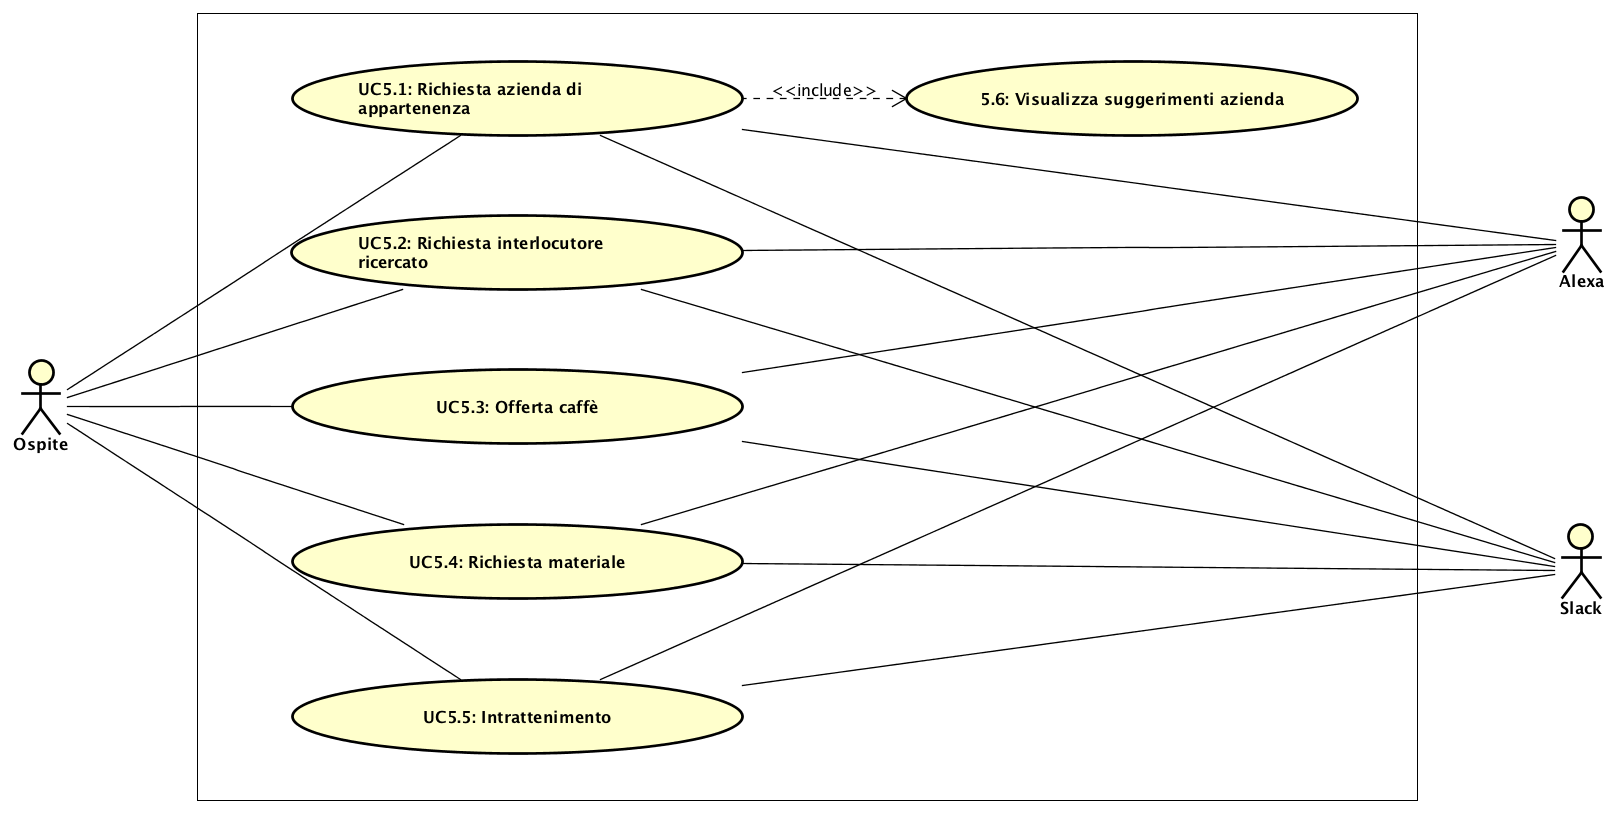
\includegraphics[width=\textwidth]{UseCases/UC5_Conversazione/UC5_Conversazione.png}
	\caption{UC5 - Conversazione}
\end{figure}
\begin{itemize} 
\item \textbf{Attori}: Alexa, Ospite, Slack.
\item \textbf{Descrizione}: l'ospite e il sistema cominciano ad interagire con una serie di domande e risposte;
\item \textbf{Precondizione}: l'utente è correttamente identificato nel sistema come ospite;
\item \textbf{Postcondizione}: il sistema ha posto le dovute domande all'ospite;
\item \textbf{Scenario principale}: \begin{enumerate}\item Richiesta azienda di appartenenza (UC5.1);\item Richiesta interlocutore ricercato (UC5.2);\item Offerta caffè (UC5.3);\item Richiesta materiale (UC5.4);\item Intrattenimento (UC5.5). 
 \end{enumerate}
\end{itemize} 
\subsection{UC5.1 - Richiesta azienda di appartenenza} 
\label{sssec:UC5.1} 
\begin{itemize} 
\item \textbf{Attori}: Alexa, Ospite, Slack.
\item \textbf{Descrizione}: il sistema chiede all'utente a quale azienda appartiene, al fine di pubblicare messaggi nel canale Slack dedicato a quella azienda, o crearlo da zero nel caso non fosse ancora stato creato;
\item \textbf{Precondizione}: Alexa è disponibile e correttamente funzionante. Slack è disponibile e correttamente funzionante. L'utente è correttamente identificato come ospite nel sistema;
\item \textbf{Postcondizione}: il sistema rimane in attesa di una risposta da parte dell'ospite;
\item \textbf{Scenario principale}: \begin{enumerate}\item Visualizza suggerimenti azienda (UC5.6). 
 \end{enumerate}
\end{itemize} 
\subsection{UC5.2 - Richiesta interlocutore ricercato} 
\label{sssec:UC5.2} 
\begin{itemize} 
\item \textbf{Attori}: Alexa, Ospite, Slack.
\item \textbf{Descrizione}: il sistema chiede all'utente quale persona stia cercando e, nel caso abbia bisogno di una persona specifica, ripropone la richiesta sul canale Slack corretto;
\item \textbf{Precondizione}: Alexa è disponibile e correttamente funzionante. Slack è disponibile e correttamente funzionante. L'utente è correttamente identificato come ospite nel sistema;
\item \textbf{Postcondizione}: il sistema rimane in attesa di una risposta da parte dell'ospite;
\item \textbf{Scenario principale}: il sistema domanda all'utente quale membro del personale interno all'azienda stia cercando;
\end{itemize} 
\subsection{UC5.3 - Offerta caffè} 
\label{sssec:UC5.3} 
\begin{itemize} 
\item \textbf{Attori}: Alexa, Ospite, Slack.
\item \textbf{Descrizione}: il sistema chiede all'utente se desidera un caffè. La risposta dell'utente viene pubblicata nel canale Slack corretto;
\item \textbf{Precondizione}: Alexa è disponibile e correttamente funzionante. Slack è disponibile e correttamente funzionante. L'utente è correttamente identificato come ospite nel sistema;
\item \textbf{Postcondizione}: il sistema rimane in attesa di una risposta da parte dell'ospite;
\item \textbf{Scenario principale}: il sistema domanda all'utente se desidera un caffè;
\end{itemize} 
\subsection{UC5.4 - Richiesta materiale} 
\label{sssec:UC5.4} 
\begin{itemize} 
\item \textbf{Attori}: Alexa, Ospite, Slack.
\item \textbf{Descrizione}: il sistema chiede all'utente se necessita del materiale. La risposta dell'utente viene pubblicata nel canale Slack corretto;
\item \textbf{Precondizione}: Alexa è disponibile e correttamente funzionante. Slack è disponibile e correttamente funzionante. L'utente è correttamente identificato come ospite nel sistema;
\item \textbf{Postcondizione}: il sistema rimane in attesa di una risposta da parte dell'ospite;
\item \textbf{Scenario principale}: il sistema domanda all'utente se necessita di qualche materiale particolare;
\end{itemize} 
\subsection{UC5.5 - Intrattenimento} 
\label{sssec:UC5.5} 
\begin{itemize} 
\item \textbf{Attori}: Alexa, Ospite, Slack.
\item \textbf{Descrizione}: il sistema propone all'utente una lista di argomenti con il quale interagire. La scelta degli argomenti viene pubblicata nel canale Slack corretto;
\item \textbf{Precondizione}: Alexa è disponibile e correttamente funzionante. Slack è disponibile e correttamente funzionante. L'utente è correttamente identificato come ospite nel sistema;
\item \textbf{Postcondizione}: il sistema rimane in attesa di una risposta da parte dell'ospite;
\item \textbf{Scenario principale}: \begin{enumerate}\item Meteo (UC5.5.1);\item News (UC5.5.2);\item Barzellette (UC5.5.3). 
 \end{enumerate}
\end{itemize} 
\subsection{UC5.5.1 - Meteo} 
\label{sssec:UC5.5.1} 
\begin{itemize} 
\item \textbf{Attori}: Alexa, Ospite.
\item \textbf{Descrizione}: il sistema chiede all'utente una località, e ne dice poi il meteo attuale;
\item \textbf{Precondizione}: l'utente ha indicato al sistema di voler proseguire con la sezione di intrattenimento;
\item \textbf{Postcondizione}: il sistema ha restituito all'ospite il meteo corrente;
\item \textbf{Scenario principale}: il sistema chiede all'utente una località, e ne descrive poi le condizioni meteo attuali;
\end{itemize} 
\subsection{UC5.5.2 - News} 
\label{sssec:UC5.5.2} 
\begin{itemize} 
\item \textbf{Attori}: Alexa, Ospite.
\item \textbf{Descrizione}: il sistema interagisce con l'utente elencando alcune news generiche recenti;
\item \textbf{Precondizione}: l'utente ha indicato al sistema di voler proseguire con la sezione di intrattenimento;
\item \textbf{Postcondizione}: il sistema ha restituito all'ospite una news;
\item \textbf{Scenario principale}: il sistema interagisce con l'utente elencando alcune news generiche recenti;
\end{itemize} 
\subsection{UC5.5.3 - Barzellette} 
\label{sssec:UC5.5.3} 
\begin{itemize} 
\item \textbf{Attori}: Alexa, Ospite.
\item \textbf{Descrizione}: il sistema interagisce con l'utente raccontando qualche barzelletta;
\item \textbf{Precondizione}: l'utente ha indicato al sistema di voler proseguire con la sezione di intrattenimento;
\item \textbf{Postcondizione}: il sistema ha restituito all'ospite una barzelletta;
\item \textbf{Scenario principale}: il sistema interagisce con l'utente raccontando delle barzellette;
\end{itemize} 
\subsection{UC5.6 - Visualizza suggerimenti azienda} 
\label{sssec:UC5.6} 
\begin{itemize} 
\item \textbf{Attori}: Ospite, Slack.
\item \textbf{Descrizione}: il sistema mostra all'utente una lista con le possibili aziende di appartenenza se l'utente si è già presentato in passato, al fine di pubblicare messaggi nel canale Slack dedicato alla propria azienda di appartenenza;
\item \textbf{Precondizione}: il sistema ha chiesto all'ospite a quale azienda appartiene;
\item \textbf{Postcondizione}: il sistema rimane in attesa di una risposta a schermo da parte dell'ospite;
\item \textbf{Scenario principale}: il sistema mostra all'utente una lista con le possibili aziende di appartenenza nel caso in cui l'utente si fosse già presentato in passato;
\end{itemize} 
\subsection{UC6 - Logout} 
\label{sssec:UC6} 
\begin{itemize} 
\item \textbf{Attori}: Admin, SuperAdmin.
\item \textbf{Descrizione}: un utente amministratore correttamente loggato nel sistema come Admin o SuperAdmin può effettuare il logout;
\item \textbf{Precondizione}: un utente amministratore è correttamente loggato nel sistema come Admin o SuperAdmin;
\item \textbf{Postcondizione}: un utente amministratore non è più loggato nel sistema;
\item \textbf{Scenario principale}: l'Admin o il SuperAdmin, se correttamente loggati nel sistema, possono effettuare il logout;
\end{itemize} 
\newpage
\subsection{UC7 - Gestione pannello Admin} 
\label{sssec:UC7} 
\begin{figure}[!h]
	\centering
	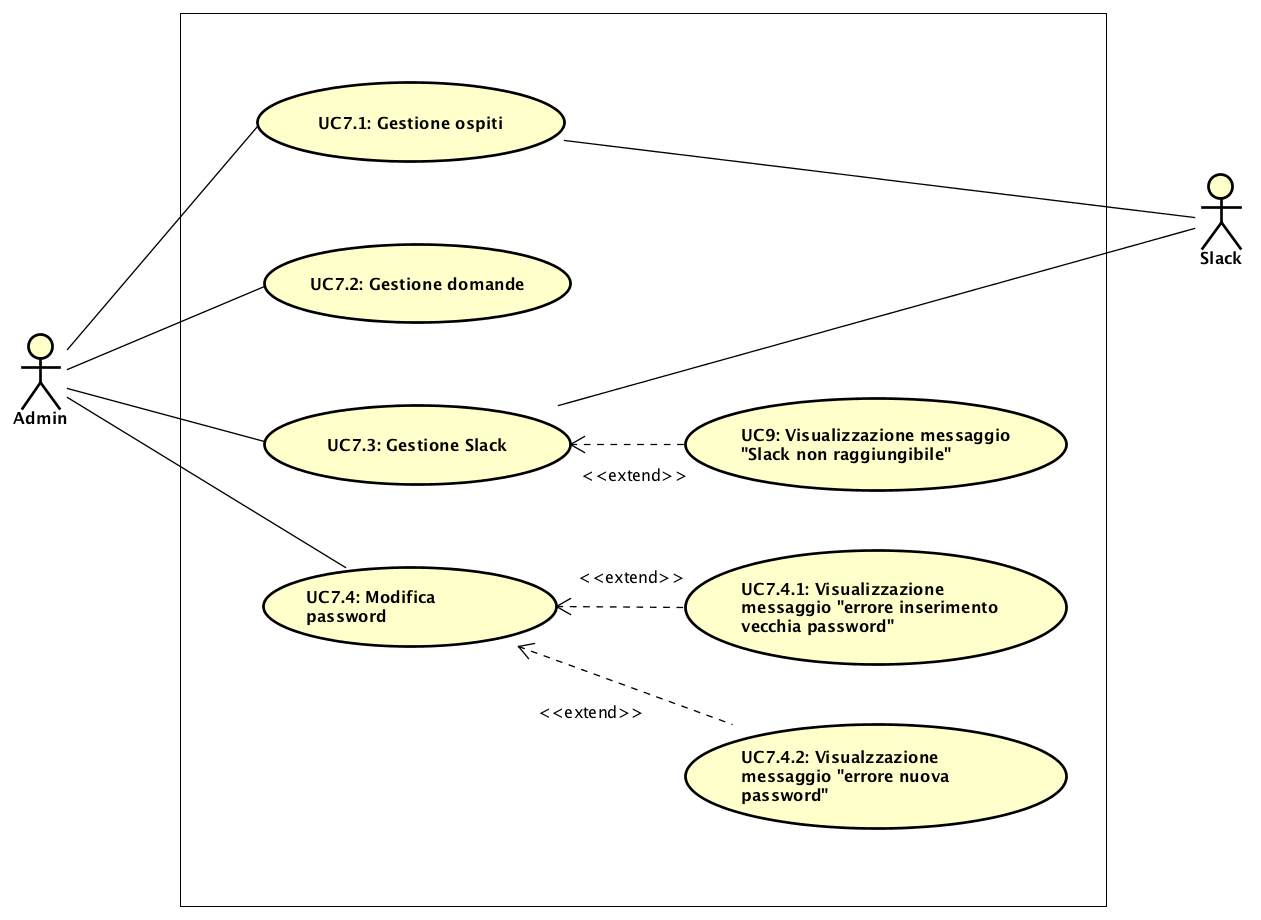
\includegraphics[width=\textwidth]{UseCases/UC7_GestionePannelloAdmin/UC7_GestionePannelloAdmin.png}
	\caption{UC7 - Gestione pannello Admin}
\end{figure}
\begin{itemize} 
\item \textbf{Attori}: Admin, SuperAdmin, Slack.
\item \textbf{Descrizione}: l'Admin può gestire il pannello dell'area amministrativa;
\item \textbf{Precondizione}: l'utente amministratore è correttamente loggato come Admin nel sistema;
\item \textbf{Postcondizione}: l'Admin ha correttamente usufruito delle funzionalità messe a disposizione dal sistema;
\item \textbf{Scenario principale}: \begin{enumerate}\item Gestione ospiti (UC7.1);\item Gestione domande (UC7.2);\item Gestione Slack (UC7.3);\item Modifica password (UC7.4). 
 \end{enumerate}
\end{itemize} 
\newpage
\subsection{UC7.1 - Gestione ospiti} 
\label{sssec:UC7.1} 
\begin{figure}[!h]
	\centering
	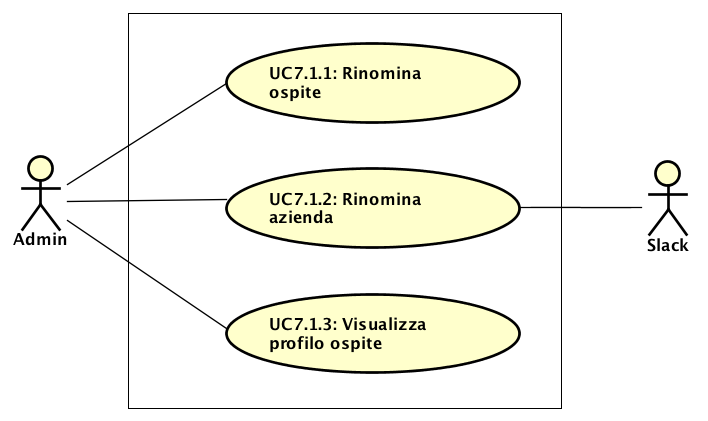
\includegraphics[width=\textwidth]{UseCases/UC7_GestionePannelloAdmin/UC7_1_GestioneOspiti/UC7_1_GestioneOspiti.png}
	\caption{UC7.1 - Gestione ospiti}
\end{figure}
\begin{itemize} 
\item \textbf{Attori}: Admin, SuperAdmin, Slack.
\item \textbf{Descrizione}: l'Admin può gestire gli ospiti presenti nel sistema;
\item \textbf{Precondizione}: l'utente amministratore è correttamente loggato come Admin nel sistema e vuole gestire gli ospiti;
\item \textbf{Postcondizione}: l'utente amministratore è riuscito a gestire correttamente gli ospiti;
\item \textbf{Scenario principale}: \begin{enumerate}\item Rinomina ospite (UC7.1.1);\item Rinomina azienda (UC7.1.2);\item Visualizza profilo ospite (UC7.1.3). 
 \end{enumerate}
\end{itemize} 
\subsection{UC7.1.1 - Rinomina ospite} 
\label{sssec:UC7.1.1} 
\begin{itemize} 
\item \textbf{Attori}: Admin, SuperAdmin.
\item \textbf{Descrizione}: l'Admin può rinominare un ospite presente nel sistema;
\item \textbf{Precondizione}: l'utente amministratore vuole rinominare un ospite;
\item \textbf{Postcondizione}: l'utente amministratore ha correttamente rinominato un ospite;
\item \textbf{Scenario principale}: l'Admin rinomina un ospite presente nel sistema;
\end{itemize} 
\subsection{UC7.1.2 - Rinomina azienda} 
\label{sssec:UC7.1.2} 
\begin{itemize} 
\item \textbf{Attori}: Admin, Slack, SuperAdmin.
\item \textbf{Descrizione}: l'Admin può rinominare l'azienda relativa ad un ospite ed allo stesso tempo viene rinominato il relativo canale \#azienda su Slack;
\item \textbf{Precondizione}: Slack è disponibile e correttamente funzionante. L'utente amministratore vuole rinominare una azienda;
\item \textbf{Postcondizione}: l'utente amministratore ha correttamente rinominato un'azienda e il relativo canale \#azienda su Slack;
\item \textbf{Scenario principale}: l'Admin rinomina l'azienda relativa ad un ospite ed allo stesso tempo viene rinominato il relativo canale \#azienda su Slack;
\end{itemize} 
\subsection{UC7.1.3 - Visualizza profilo ospite} 
\label{sssec:UC7.1.3} 
\begin{itemize} 
\item \textbf{Attori}: Admin, SuperAdmin.
\item \textbf{Descrizione}: l'Admin può visualizzare il profilo di un ospite presente nel sistema con le sue relative informazioni quali, ad esempio, se è solito a bere un caffè, se di solito necessita di qualche materiale, e tutte le altre informazioni che il sistema riesce a raccogliere in base alle domande che effettua;
\item \textbf{Precondizione}: l'utente amministratore vuole visualizzare il profilo di un ospite;
\item \textbf{Postcondizione}: l'utente amministratore ha correttamente visualizzato il profilo di un ospite;
\item \textbf{Scenario principale}: l'Admin visualizza il profilo di un ospite presente nel sistema con le sue relative informazioni;
\end{itemize}

\newpage
\subsection{UC7.2 - Gestione domande} 
\label{sssec:UC7.2} 
\begin{figure}[!h]
	\centering
	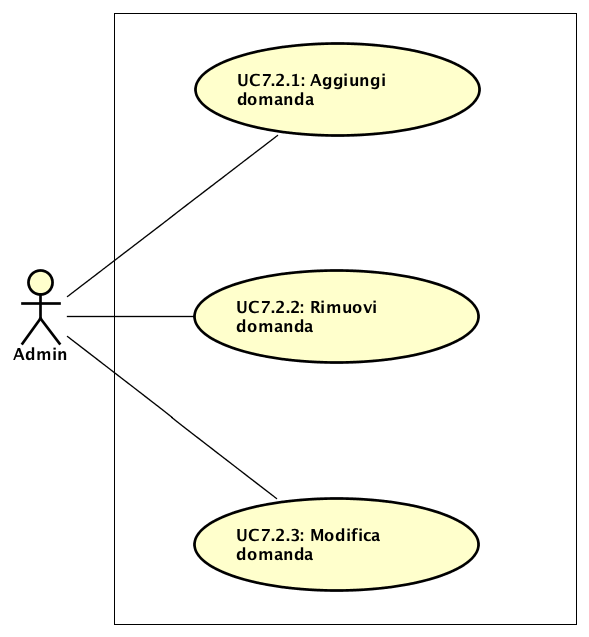
\includegraphics[width=\textwidth]{UseCases/UC7_GestionePannelloAdmin/UC7_2_GestioneDomande/UC7_2_GestioneDomande.png}
	\caption{UC7.2 - Gestione domande}
\end{figure}
\begin{itemize} 
\item \textbf{Attori}: Admin, SuperAdmin.
\item \textbf{Descrizione}: l'Admin può gestire le domande che il sistema può porre all'ospite;
\item \textbf{Precondizione}: l'utente amministratore è correttamente loggato come Admin nel sistema e vuole gestire le domande;
\item \textbf{Postcondizione}: l'utente amministratore è riuscito a gestire correttamente le domande;
\item \textbf{Scenario principale}: \begin{enumerate}\item Aggiungi domanda (UC7.2.1);\item Rimuovi domanda (UC7.2.2);\item Modifica domanda (UC7.2.3).
\end{enumerate}
\end{itemize} 
\subsection{UC7.2.1 - Aggiungi domanda} 
\label{sssec:UC7.2.1} 
\begin{figure}[!h]
	\centering
	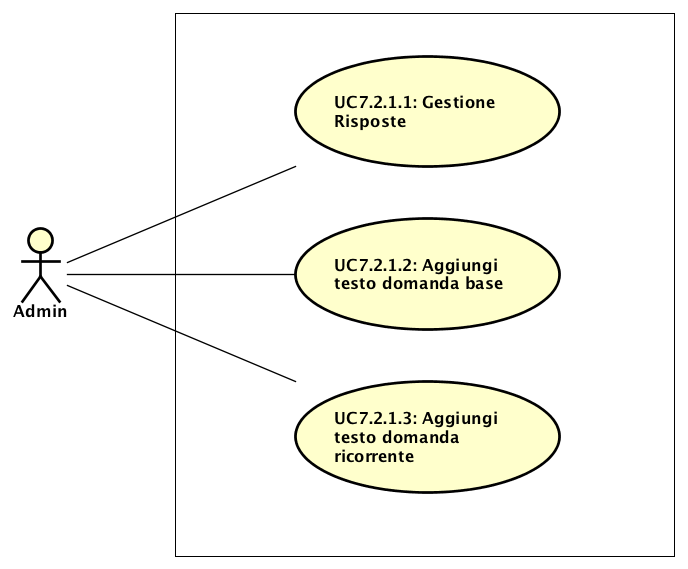
\includegraphics[scale=0.7]{UseCases/UC7_GestionePannelloAdmin/UC7_2_GestioneDomande/UC7_2_1_AggiungiDomanda/UC7_2_1_AggiungiDomanda.png}
	\caption{UC7.2.1 - Aggiungi domanda}
\end{figure}
\begin{itemize} 
\item \textbf{Attori}: Admin, SuperAdmin.
\item \textbf{Descrizione}: l'Admin può aggiungere una domanda che il sistema porrà all'ospite;
\item \textbf{Precondizione}: l'utente amministratore vuole aggiungere una domanda;
\item \textbf{Postcondizione}: l'utente amministratore ha correttamente aggiunto una domanda;
\item \textbf{Scenario principale}: \begin{enumerate}\item Gestione Risposte (UC7.2.4);\item Aggiungi testo domanda base (UC7.2.1.2);\item Aggiungi testo domanda ricorrente (UC7.2.1.3).
\end{enumerate}
\newpage
\subsection{UC7.2.1.1 - Gestione risposte} 
\label{sssec:UC7.2.1.1} 
\begin{figure}[!h]
	\centering
	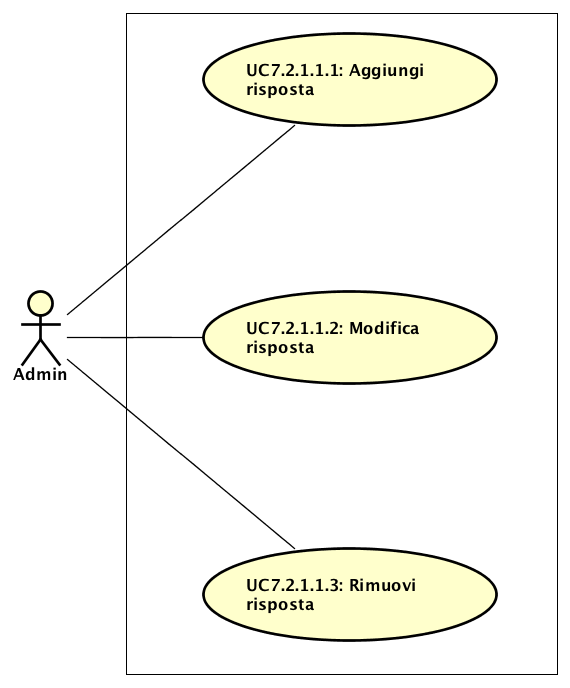
\includegraphics[scale=0.7]{UseCases/UC7_GestionePannelloAdmin/UC7_2_GestioneDomande/UC7_2_1_AggiungiDomanda/UC7_2_1_1_GestioneRisposte/UC7_2_1_1_GestioneRisposte.png}
	\caption{UC7.2.1.1 - Gestione risposte}
\end{figure}
\begin{itemize} 
\item \textbf{Attori}: Admin, SuperAdmin.
\item \textbf{Descrizione}: l'Admin può gestire le risposte che il sistema può accettare da un ospite in base alla relativa domanda;
\item \textbf{Precondizione}: l'utente amministratore vuole gestire le risposte per aggiungere la domanda;
\item \textbf{Postcondizione}: l'utente amministratore è riuscito a gestire correttamente le risposte;
\item \textbf{Scenario principale}: \begin{enumerate}\item Aggiungi risposta (UC7.2.1.1.1);\item Modifica risposta (UC7.2.1.1.2);\item Rimuovi risposta (UC7.2.1.1.3).
 \end{enumerate}
\end{itemize}  
\newpage
\subsection{UC7.2.1.1.1 - Aggiungi risposta} 
\label{sssec:UC7.2.1.1.1} 
\begin{figure}[!h]
	\centering
	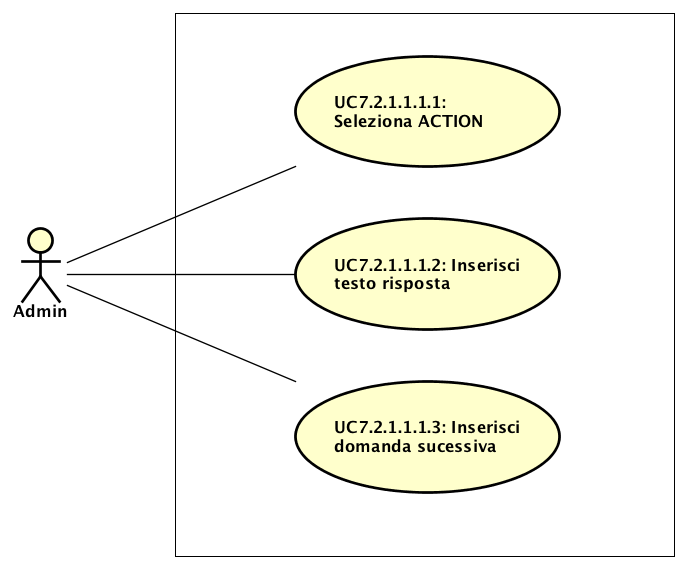
\includegraphics[scale=0.7]{UseCases/UC7_GestionePannelloAdmin/UC7_2_GestioneDomande/UC7_2_1_AggiungiDomanda/UC7_2_1_1_GestioneRisposte/UC7_2_1_1_1_AggiungiRisposta/UC7_2_1_1_1_AggiungiRisposta.png}
	\caption{UC7.2.1.1.1 - Aggiungi risposta}
\end{figure}
\begin{itemize} 
\item \textbf{Attori}: Admin, SuperAdmin.
\item \textbf{Descrizione}: l'Admin può aggiungere una risposta che il sistema può accettare;
\item \textbf{Precondizione}: l'utente amministratore vuole aggiungere una risposta;
\item \textbf{Postcondizione}: l'utente amministratore ha correttamente aggiunto una risposta;
\item \textbf{Scenario principale}: \begin{enumerate}\item Seleziona ACTION (UC7.2.1.1.1.1);\item Inserisci testo risposta (UC7.2.1.1.1.2);\item Inserisci domanda successiva (UC7.2.1.1.1.3).
\end{enumerate}
\end{itemize}  
\subsection{UC7.2.1.1.1.1 - Seleziona ACTION} 
\label{sssec:UC7.2.1.1.1.1} 
\begin{itemize} 
\item \textbf{Attori}: Admin, SuperAdmin.
\item \textbf{Descrizione}: l'Admin può associare ad una risposta una ACTION predefinita da sistema, selezionandone una tra quelle presenti;
\item \textbf{Precondizione}: l'utente amministratore vuole associare una ACTION ad una risposta tra quelle disponibili;
\item \textbf{Postcondizione}: l'utente amministratore ha correttamente associato una ACTION ad una risposta;\item \textbf{Scenario principale}: l'Admin associa ad una risposta una ACTION predefinita da sistema, selezionandone una tra quelle presenti;
\end{itemize} 
\subsection{UC7.2.1.1.1.2 - Inserisci testo risposta} 
\label{sssec:UC7.2.1.1.1.2} 
\begin{itemize} 
\item \textbf{Attori}: Admin, SuperAdmin.
\item \textbf{Descrizione}: l'Admin può aggiungere il testo della risposta che il sistema può accettare dall'ospite;
\item \textbf{Precondizione}: l'utente amministratore vuole aggiungere il testo della risposta;
\item \textbf{Postcondizione}: l'utente amministratore è riuscito ad inserire correttamente il testo della risposta;
\item \textbf{Scenario principale}: l'Admin inserisce il testo della risposta che il sistema può accettare dall'ospite;
\end{itemize} 
\subsection{UC7.2.1.1.1.3 - Inserisci domanda successiva} 
\label{sssec:UC7.2.1.1.1.2} 
\begin{itemize} 
\item \textbf{Attori}: Admin, SuperAdmin.
\item \textbf{Descrizione}: l'Admin può aggiungere la domanda successiva che il sistema porrà all'ospite, selezionandone una dalla lista delle domande presenti nel sistema;
\item \textbf{Precondizione}: l'utente amministratore vuole aggiungere una domanda successiva alla corrente;
\item \textbf{Postcondizione}: l'utente amministratore ha correttamente aggiunto una domanda successiva alla corrente;
\item \textbf{Scenario principale}: l'Admin aggiunge la domanda successiva che il sistema porrà all'ospite;
\end{itemize} 
\newpage
\subsection{UC7.2.1.1.2 - Modifica risposta} 
\label{sssec:UC7.2.1.1.2} 
\begin{figure}[!h]
	\centering
	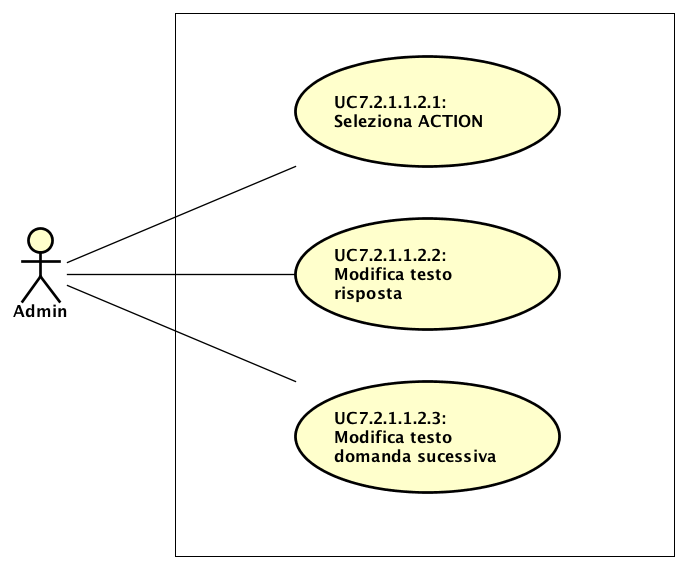
\includegraphics[scale=0.7]{UseCases/UC7_GestionePannelloAdmin/UC7_2_GestioneDomande/UC7_2_1_AggiungiDomanda/UC7_2_1_1_GestioneRisposte/UC7_2_1_1_2_ModificaRisposta/UC7_2_1_1_2_ModificaRisposta.png}
	\caption{UC7.2.1.1.2 - Modifica risposta}
\end{figure}
\begin{itemize} 
\item \textbf{Attori}: Admin, SuperAdmin.
\item \textbf{Descrizione}: l'Admin può modificare una risposta che il sistema può accettare;
\item \textbf{Precondizione}: l'utente amministratore vuole modificare una risposta;
\item \textbf{Postcondizione}: l'utente amministratore ha correttamente modificato una risposta;
\item \textbf{Scenario principale}: \begin{enumerate}\item Seleziona ACTION (UC7.2.1.1.2.1);\item Modifica testo risposta (UC7.2.1.1.2.2);\item Modifica domanda successiva (UC7.2.1.1.2.3).
\end{enumerate}
\end{itemize} 
\subsection{UC7.2.1.1.2.1 - Seleziona ACTION} 
\label{sssec:UC7.2.1.1.2.1} 
\begin{itemize} 
\item \textbf{Attori}: Admin, SuperAdmin.
\item \textbf{Descrizione}: l'Admin può associare ad una risposta una ACTION predefinita da sistema, selezionandone una tra quelle presenti;
\item \textbf{Precondizione}: l'utente amministratore vuole associare una ACTION ad una risposta tra quelle disponibili;
\item \textbf{Postcondizione}: l'utente amministratore ha correttamente associato una ACTION ad una risposta;\item \textbf{Scenario principale}: l'Admin associa ad una risposta una ACTION predefinita da sistema, selezionandone una tra quelle presenti;
\end{itemize}
\subsection{UC7.2.1.1.2.2 - Modifica testo risposta} 
\label{sssec:UC7.2.1.1.2.2} 
\begin{itemize} 
\item \textbf{Attori}: Admin, SuperAdmin.
\item \textbf{Descrizione}: l'Admin può modificare il testo della risposta che il sistema può accettare dall'ospite;
\item \textbf{Precondizione}: l'utente amministratore vuole modificare il testo della risposta;
\item \textbf{Postcondizione}: l'utente amministratore è riuscito a modificare correttamente il testo della risposta;
\item \textbf{Scenario principale}: l'Admin modifica il testo della risposta che il sistema può accettare dall'ospite;
\end{itemize} 
\subsection{UC7.2.1.1.2.3 - Modifica domanda successiva} 
\label{sssec:UC7.2.1.1.2.3} 
\begin{itemize} 
\item \textbf{Attori}: Admin, SuperAdmin.
\item \textbf{Descrizione}: l'Admin può aggiungere o modificare la domanda successiva che il sistema porrà all'ospite, selezionandone una dalla lista delle domande presenti nel sistema;
\item \textbf{Precondizione}: l'utente amministratore vuole aggiungere una domanda successiva alla corrente;
\item \textbf{Postcondizione}: l'utente amministratore ha correttamente aggiunto una domanda successiva alla corrente;
\item \textbf{Scenario principale}: l'Admin aggiunge o modifica la domanda successiva che il sistema porrà all'ospite;
\end{itemize} 
\subsection{UC7.2.1.1.3 - Rimuovi risposta} 
\label{sssec:UC7.2.1.1.3} 
\begin{itemize} 
\item \textbf{Attori}: Admin, SuperAdmin.
\item \textbf{Descrizione}: l'Admin può rimuovere una risposta che il sistema può accettare;
\item \textbf{Precondizione}: l'utente amministratore vuole rimuovere una risposta;
\item \textbf{Postcondizione}: l'utente amministratore ha correttamente rimosso una risposta;
\item \textbf{Scenario principale}: l'Admin rimuove una risposta che il sistema può accettare;
\end{itemize}
\subsection{UC7.2.1.2 - Aggiungi testo domanda base} 
\label{sssec:UC7.2.1.2} 
\begin{itemize} 
\item \textbf{Attori}: Admin, SuperAdmin.
\item \textbf{Descrizione}: l'Admin può inserire il testo della domanda base, cioè la domanda che verrà posta all'ospite se è la sua prima visita;
\item \textbf{Precondizione}: l'utente amministratore vuole inserire il testo della domanda base;
\item \textbf{Postcondizione}: l'utente amministratore è riuscito ad inserire correttamente il testo della domanda;
\item \textbf{Descrizione}: l'Admin inserisce il testo della domanda base;
\end{itemize} 
\subsection{UC7.2.1.3 - Aggiungi testo domanda ricorrente} 
\label{sssec:UC7.2.1.3} 
\begin{itemize} 
\item \textbf{Attori}: Admin, SuperAdmin.
\item \textbf{Descrizione}: l'Admin può inserire il testo della domanda ricorrente, cioè la domanda che verrà posta all'ospite se non è la sua prima visita;
\item \textbf{Precondizione}: l'utente amministratore vuole inserire il testo della domanda ricorrente;
\item \textbf{Postcondizione}: l'utente amministratore è riuscito ad inserire correttamente il testo della domanda;
\item \textbf{Scenario principale}: l'Admin inserisce il testo della domanda ricorrente;
\end{itemize} 
\end{itemize} 
\subsection{UC7.2.2 - Rimuovi domanda} 
\label{sssec:UC7.2.2} 
\begin{itemize} 
\item \textbf{Attori}: Admin, SuperAdmin.
\item \textbf{Descrizione}: l'Admin può rimuovere una domanda tra quelle che il sistema porrà all'ospite;
\item \textbf{Precondizione}: l'utente amministratore vuole rimuovere una domanda;
\item \textbf{Postcondizione}: l'utente amministratore ha correttamente rimosso una domanda;
\item \textbf{Scenario principale}: l'Admin rimuove una domanda tra quelle che il sistema potrà porre all'ospite;
\end{itemize} 
%SEI ARRIVATO QUI
\newpage
\subsection{UC7.2.3 - Modifica domanda} 
\label{sssec:UC7.2.3} 
\begin{figure}[!h]
	\centering
	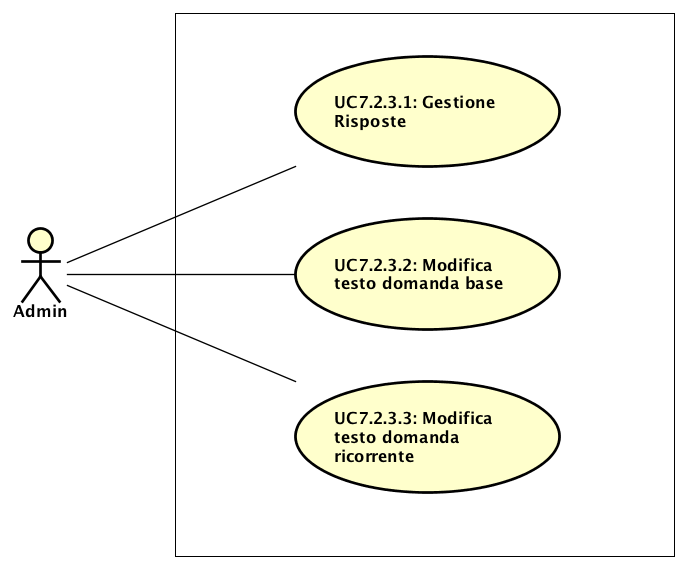
\includegraphics[scale=0.7]{UseCases/UC7_GestionePannelloAdmin/UC7_2_GestioneDomande/UC7_2_3_ModificaDomanda/UC7_2_3_ModificaDomanda.png}
	\caption{UC7.2.3 - Modifica domanda}
\end{figure}
\begin{itemize} 
\item \textbf{Attori}: Admin, SuperAdmin.
\item \textbf{Descrizione}: l'Admin può modificare una domanda tra quelle che il sistema porrà all'ospite;
\item \textbf{Precondizione}: l'utente amministratore vuole modificare una domanda;
\item \textbf{Postcondizione}: l'utente amministratore ha correttamente modificato una domanda;
\item \textbf{Scenario principale}: \begin{enumerate}\item Gestione Risposte (UC7.2.3.1);\item Modifica testo domanda base (UC7.2.3.2);\item Modifica testo domanda ricorrente (UC7.2.3.3).
\end{enumerate}
\end{itemize} 
\newpage
\subsection{UC7.2.3.1 - Gestione risposte} 
\label{sssec:UC7.2.3.1} 
\begin{figure}[!h]
	\centering
	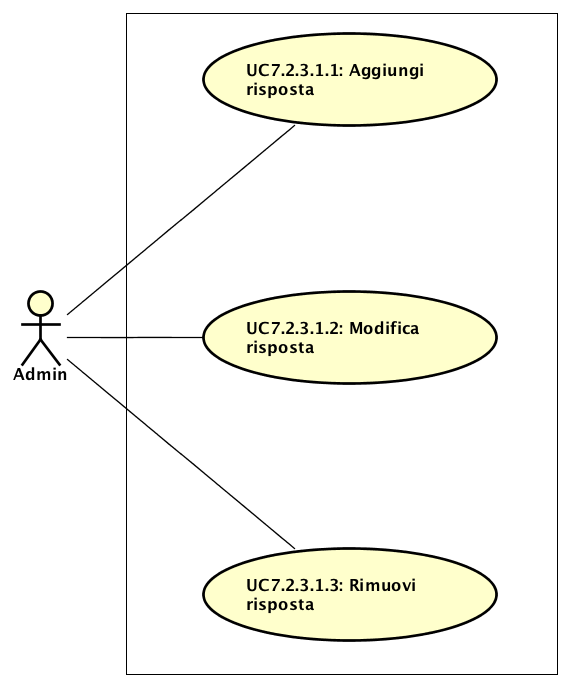
\includegraphics[scale=0.7]{UseCases/UC7_GestionePannelloAdmin/UC7_2_GestioneDomande/UC7_2_3_ModificaDomanda/UC7_2_3_1_GestioneRisposte/UC7_2_3_1_GestioneRisposte.png}
	\caption{UC7.2.3.1 - Gestione risposte}
\end{figure}
\begin{itemize} 
\item \textbf{Attori}: Admin, SuperAdmin.
\item \textbf{Descrizione}: l'Admin può gestire le risposte che il sistema può accettare da un ospite in base alla relativa domanda;
\item \textbf{Precondizione}: l'utente amministratore vuole gestire le risposte modificando una domanda;
\item \textbf{Postcondizione}: l'utente amministratore è riuscito a gestire correttamente le risposte;
\item \textbf{Scenario principale}: \begin{enumerate}\item Aggiungi risposta (UC7.2.3.1.1);\item Modifica risposta (UC7.2.3.1.2);\item Rimuovi risposta (UC7.2.3.1.3).
 \end{enumerate}
\end{itemize} 
\newpage
\subsection{UC7.2.3.1.1 - Aggiungi risposta} 
\label{sssec:UC7.2.3.1.1} 
\begin{figure}[!h]
	\centering
	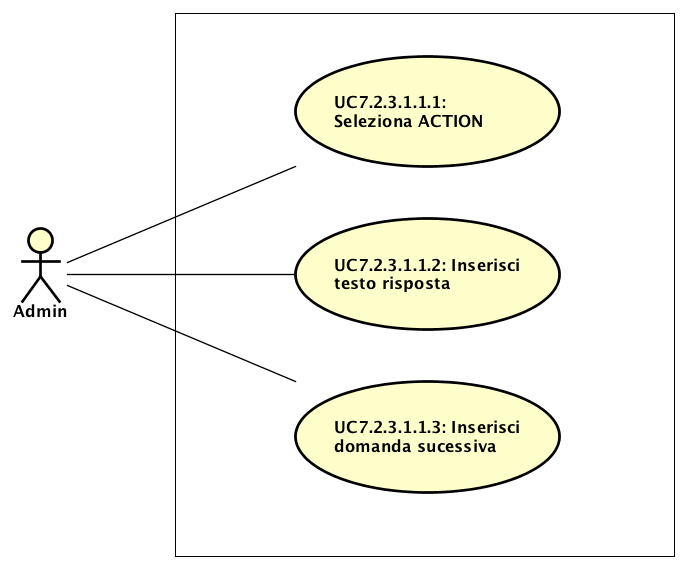
\includegraphics[scale=0.7]{UseCases/UC7_GestionePannelloAdmin/UC7_2_GestioneDomande/UC7_2_3_ModificaDomanda/UC7_2_3_1_GestioneRisposte/UC7_2_3_1_1_AggiungiRisposta/UC7_2_3_1_1_AggiungiRisposta.png}
	\caption{UC7.2.4.1 - Aggiungi risposta}
\end{figure}
\begin{itemize} 
\item \textbf{Attori}: Admin, SuperAdmin.
\item \textbf{Descrizione}: l'Admin può aggiungere una risposta che il sistema può accettare;
\item \textbf{Precondizione}: l'utente amministratore vuole aggiungere una risposta;
\item \textbf{Postcondizione}: l'utente amministratore ha correttamente aggiunto una risposta;
\item \textbf{Scenario principale}: \begin{enumerate}\item Seleziona ACTION (UC7.2.3.1.1.1);\item Inserisci testo risposta (UC7.2.3.1.1.2);\item Inserisci domanda successiva (UC7.2.3.1.1.3).
\end{enumerate}
\end{itemize}  
\subsection{UC7.2.3.1.1.1 - Seleziona ACTION} 
\label{sssec:UC7.2.3.1.1.1} 
\begin{itemize} 
\item \textbf{Attori}: Admin, SuperAdmin.
\item \textbf{Descrizione}: l'Admin può associare ad una risposta una ACTION predefinita da sistema, selezionandone una tra quelle presenti;
\item \textbf{Precondizione}: l'utente amministratore vuole associare una ACTION ad una risposta tra quelle disponibili;
\item \textbf{Postcondizione}: l'utente amministratore ha correttamente associato una ACTION ad una risposta;\item \textbf{Scenario principale}: l'Admin associa ad una risposta una ACTION predefinita da sistema, selezionandone una tra quelle presenti;
\end{itemize} 
\subsection{UC7.2.3.1.1.2 - Inserisci testo risposta} 
\label{sssec:UC7.2.3.1.1.2} 
\begin{itemize} 
\item \textbf{Attori}: Admin, SuperAdmin.
\item \textbf{Descrizione}: l'Admin può aggiungere il testo della risposta che il sistema può accettare dall'ospite;
\item \textbf{Precondizione}: l'utente amministratore vuole aggiungere il testo della risposta;
\item \textbf{Postcondizione}: l'utente amministratore è riuscito ad inserire correttamente il testo della risposta;
\item \textbf{Scenario principale}: l'Admin inserisce il testo della risposta che il sistema può accettare dall'ospite;
\end{itemize} 
\subsection{UC7.2.3.1.1.3 - Inserisci domanda successiva} 
\label{sssec:UC7.2.3.1.1.3} 
\begin{itemize} 
\item \textbf{Attori}: Admin, SuperAdmin.
\item \textbf{Descrizione}: l'Admin può aggiungere la domanda successiva che il sistema porrà all'ospite, selezionandone una dalla lista delle domande presenti nel sistema;
\item \textbf{Precondizione}: l'utente amministratore vuole aggiungere una domanda successiva alla corrente;
\item \textbf{Postcondizione}: l'utente amministratore ha correttamente aggiunto una domanda successiva alla corrente;
\item \textbf{Scenario principale}: l'Admin aggiunge la domanda successiva che il sistema porrà all'ospite;
\end{itemize} 
\newpage
\subsection{UC7.2.3.1.2 - Modifica risposta} 
\label{sssec:UC7.2.3.1.2} 
\begin{figure}[!h]
	\centering
	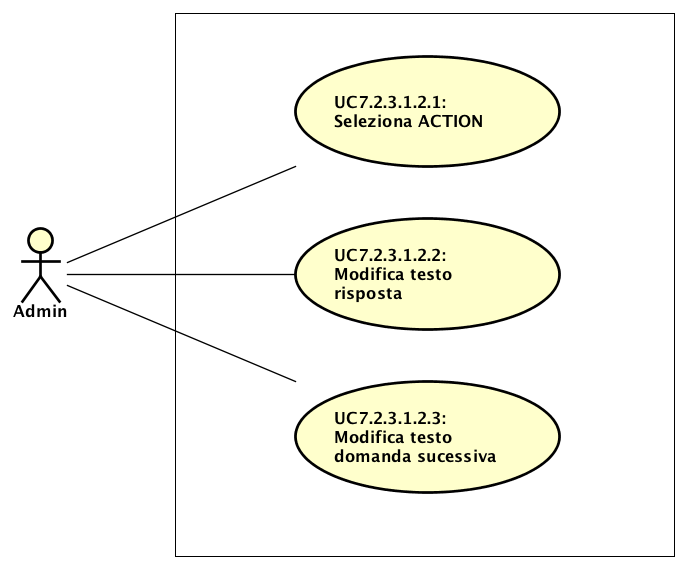
\includegraphics[scale=0.7]{UseCases/UC7_GestionePannelloAdmin/UC7_2_GestioneDomande/UC7_2_3_ModificaDomanda/UC7_2_3_1_GestioneRisposte/UC7_2_3_1_2_ModificaRisposta/UC7_2_3_1_2_ModificaRisposta.png}
	\caption{UC7.2.3.1.2 - Modifica risposta}
\end{figure}
\begin{itemize} 
\item \textbf{Attori}: Admin, SuperAdmin.
\item \textbf{Descrizione}: l'Admin può modificare una risposta che il sistema può accettare;
\item \textbf{Precondizione}: l'utente amministratore vuole modificare una risposta;
\item \textbf{Postcondizione}: l'utente amministratore ha correttamente modificato una risposta;
\item \textbf{Scenario principale}: \begin{enumerate}\item Seleziona ACTION (UC7.2.3.1.2.1);\item Modifica testo risposta (UC7.2.3.1.2.2);\item Modifica domanda successiva (UC7.2.3.1.2.3).
\end{enumerate}
\end{itemize} 
\subsection{UC7.2.3.1.2.2 - Modifica testo risposta} 
\label{sssec:UC7.2.3.1.2.2} 
\begin{itemize} 
\item \textbf{Attori}: Admin, SuperAdmin.
\item \textbf{Descrizione}: l'Admin può modificare il testo della risposta che il sistema può accettare dall'ospite;
\item \textbf{Precondizione}: l'utente amministratore vuole modificare il testo della risposta;
\item \textbf{Postcondizione}: l'utente amministratore è riuscito a modificare correttamente il testo della risposta;
\item \textbf{Scenario principale}: l'Admin modifica il testo della risposta che il sistema può accettare dall'ospite;
\end{itemize} 
\subsection{UC7.2.3.1.2.3 - Modifica domanda successiva} 
\label{sssec:UC7.2.3.1.2.3} 
\begin{itemize} 
\item \textbf{Attori}: Admin, SuperAdmin.
\item \textbf{Descrizione}: l'Admin può aggiungere o modificare la domanda successiva che il sistema porrà all'ospite, selezionandone una dalla lista delle domande presenti nel sistema;
\item \textbf{Precondizione}: l'utente amministratore vuole aggiungere una domanda successiva alla corrente;
\item \textbf{Postcondizione}: l'utente amministratore ha correttamente aggiunto una domanda successiva alla corrente;
\item \textbf{Scenario principale}: l'Admin aggiunge o modifica la domanda successiva che il sistema porrà all'ospite;
\end{itemize} 
\subsection{UC7.2.3.1.3 - Rimuovi risposta} 
\label{sssec:UC7.2.3.1.3} 
\begin{itemize} 
\item \textbf{Attori}: Admin, SuperAdmin.
\item \textbf{Descrizione}: l'Admin può rimuovere una risposta che il sistema può accettare;
\item \textbf{Precondizione}: l'utente amministratore vuole rimuovere una risposta;
\item \textbf{Postcondizione}: l'utente amministratore ha correttamente rimosso una risposta;
\item \textbf{Scenario principale}: l'Admin rimuove una risposta che il sistema può accettare;
\end{itemize}
\subsection{UC7.2.3.2 - Modifica testo domanda base} 
\label{sssec:UC7.2.3.2} 
\begin{itemize} 
\item \textbf{Attori}: Admin, SuperAdmin.
\item \textbf{Descrizione}: l'Admin può modificare il testo della domanda base, cioè la domanda che verrà posta all'ospite se è la sua prima visita;
\item \textbf{Precondizione}: l'utente amministratore vuole modificare il testo della domanda base;
\item \textbf{Postcondizione}: l'utente amministratore è riuscito a modificare correttamente il testo della domanda;
\item \textbf{Descrizione}: l'Admin modifica il testo della domanda base;
\end{itemize} 
\subsection{UC7.2.3.3 - Modifica testo domanda ricorrente} 
\label{sssec:UC7.2.3.3} 
\begin{itemize} 
\item \textbf{Attori}: Admin, SuperAdmin.
\item \textbf{Descrizione}: l'Admin può modificare il testo della domanda ricorrente, cioè la domanda che verrà posta all'ospite se non è la sua prima visita;
\item \textbf{Precondizione}: l'utente amministratore vuole modificare il testo della domanda ricorrente;
\item \textbf{Postcondizione}: l'utente amministratore è riuscito a modificare correttamente il testo della domanda;
\item \textbf{Scenario principale}: l'Admin modifica il testo della domanda ricorrente;
\end{itemize}
\newpage
\subsection{UC7.3 - Gestione Slack} 
\label{sssec:UC7.3} 
\begin{figure}[!h]
	\centering
	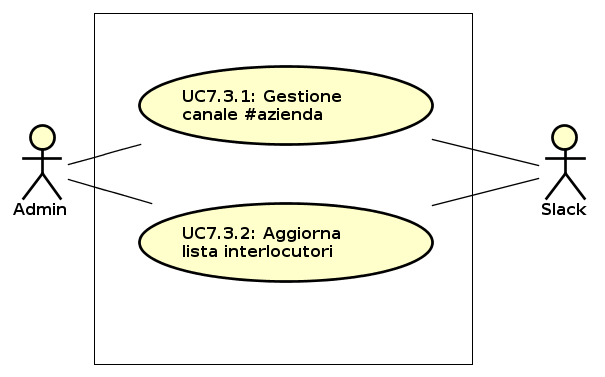
\includegraphics[width=\textwidth]{UseCases/UC7_GestionePannelloAdmin/UC7_3_GestioneSlack/UC7_3_GestioneSlack.png}
	\caption{UC7.3 - Gestione Slack}
\end{figure}
\begin{itemize} 
\item \textbf{Attori}: Admin, SuperAdmin, Slack.
\item \textbf{Descrizione}: l'Admin può gestire alcune impostazioni di Slack;
\item \textbf{Precondizione}: l'utente amministratore è correttamente loggato come Admin nel sistema e vuole gestire le impostazioni di Slack;
\item \textbf{Postcondizione}: l'utente amministratore è riuscito a gestire correttamente le impostazioni di Slack;
\item \textbf{Scenario principale}: \begin{enumerate}\item Gestione canale \#azienda (UC7.3.1);\item Aggiorna lista interlocutori (UC7.3.2). 
\end{enumerate}
\end{itemize} 
\subsection{UC7.3.1 - Gestione canale \#azienda} 
\label{sssec:UC7.3.1} 
\begin{itemize} 
\item \textbf{Attori}: Admin, SuperAdmin.
\item \textbf{Descrizione}: l'Admin può gestire una lista di interlocutori che verranno aggiunti di default nei canali Slack \#azienda che verranno creati;
\item \textbf{Precondizione}: l'utente amministratore vuole gestire il canale \#azienda;
\item \textbf{Postcondizione}: l'utente amministratore è riuscito a gestire correttamente il canale \#azienda;
\item \textbf{Scenario principale}: \begin{enumerate}\item Associa interlocutore (UC7.3.1.1);\item Disassocia interlocutore (UC7.3.1.2). 
 \end{enumerate}
\end{itemize} 
\subsection{UC7.3.1.1 - Associa interlocutore} 
\label{sssec:UC7.3.1.1} 
\begin{itemize} 
\item \textbf{Attori}: Admin, SuperAdmin.
\item \textbf{Descrizione}: l'Admin può associare un interlocutore alla lista degli interlocutori presente nel sistema;
\item \textbf{Precondizione}: l'utente amministratore vuole associare un interlocutore ad un canale \#azienda;
\item \textbf{Postcondizione}: l'utente amministratore è riuscito ad associare correttamente un interlocutore ad un canale \#azienda;
\item \textbf{Scenario principale}: l'Admin aggiunge un interlocutore alla lista degli interlocutori presente nel sistema;
\end{itemize} 
\subsection{UC7.3.1.2 - Disassocia interlocutore} 
\label{sssec:UC7.3.1.2} 
\begin{itemize} 
\item \textbf{Attori}: Admin, SuperAdmin.
\item \textbf{Descrizione}: l'Admin può togliere un interlocutore tra quelli presenti dalla lista;
\item \textbf{Precondizione}: l'utente amministratore vuole disassociare un interlocutore ad un canale \#azienda;
\item \textbf{Postcondizione}: l'utente amministratore è riuscito a disassociare correttamente un interlocutore ad un canale \#azienda;
\item \textbf{Scenario principale}: l'Admin toglie un interlocutore tra quelli presenti dalla lista;
\end{itemize} 
\subsection{UC7.3.2 - Aggiorna lista interlocutori} 
\label{sssec:UC7.3.2} 
\begin{itemize} 
\item \textbf{Attori}: Admin, Slack, SuperAdmin.
\item \textbf{Descrizione}: l'Admin può aggiornare la lista degli interlocutori presenti nel sistema attraverso una richiesta a Slack;
\item \textbf{Precondizione}: Slack è disponibile e correttamente funzionante. L'utente amministratore vuole gestire la lista di interlocutori;
\item \textbf{Postcondizione}: l'utente amministratore ha correttamente gestito la lista di interlocutori;
\item \textbf{Scenario principale}: l'Admin aggiorna la lista degli interlocutori presenti nel sistema attraverso una richiesta a Slack;
\end{itemize} 
\subsection{UC7.4 - Modifica password} 
\label{sssec:UC7.4} 
\begin{itemize} 
\item \textbf{Attori}: Admin, SuperAdmin.
\item \textbf{Descrizione}: l'Admin può modificare e aggiornare la propria password di accesso al sistema;
\item \textbf{Precondizione}: l'utente amministratore vuole modificare la propria password;
\item \textbf{Postcondizione}: l'utente amministratore è riuscito a modificare correttamente la propria password;
\item \textbf{Scenario principale}: \begin{enumerate}\item Visualizzazione messaggio "Errore inserimento vecchia password" (UC7.5);\item Visualizzazione messaggio "Errore nuova password" (UC7.6). 
 \end{enumerate}
\end{itemize} 
\subsection{UC7.5 - Visualizzazione messaggio "Errore inserimento vecchia password"} 
\label{sssec:UC7.5} 
\begin{itemize} 
\item \textbf{Attori}: Admin, SuperAdmin.
\item \textbf{Descrizione}: il sistema mostra un messaggio di errore perché la vecchia password inserita dall'Admin non corrisponde;
\item \textbf{Precondizione}: l'utente amministratore ha confermato di voler modificare la propria password;
\item \textbf{Postcondizione}: l'utente amministratore visualizza un messaggio di errore. Il sistema consente all'amministratore di modificare le informazioni inserite;
\item \textbf{Scenario principale}: il sistema mostra all'Admin un messaggio di errore causato dall'errato inserimento della vecchia password;
\end{itemize} 
\subsection{UC7.6 - Visualizzazione messaggio "Errore nuova password"} 
\label{sssec:UC7.6} 
\begin{itemize} 
\item \textbf{Attori}: Admin, SuperAdmin.
\item \textbf{Descrizione}: il sistema mostra un messaggio di errore perché la nuova password e la conferma della nuova password non corrispondono;
\item \textbf{Precondizione}: l'utente amministratore ha confermato di voler modificare la propria password;
\item \textbf{Postcondizione}: l'utente amministratore visualizza un messaggio di errore. Il sistema consente all'amministratore di modificare le informazioni inserite;
\item \textbf{Scenario principale}: il sistema mostra all'Admin un messaggio di errore causato dall'errata corrispondenza fra la nuova password inserita e la sua conferma;

\end{itemize} 
\newpage
\subsection{UC8 - Gestione pannello SuperAdmin} 
\label{sssec:UC8} 
\begin{figure}[!h]
	\centering
	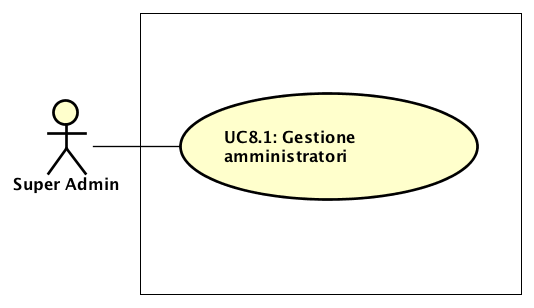
\includegraphics[width=\textwidth]{UseCases/UC8_GestionePannelloSuperadmin/UC8_GestionePannelloSuperadmin.png}
	\caption{UC8 - Gestione pannello SuperAdmin}
\end{figure}
\begin{itemize} 
\item \textbf{Attori}: SuperAdmin.
\item \textbf{Descrizione}: il SuperAdmin può gestire impostazioni extra rispetto ad un Admin normale;
\item \textbf{Precondizione}: l'utente amministratore è correttamente loggato come SuperAdmin nel sistema;
\item \textbf{Postcondizione}: il SuperAdmin ha correttamente usufruito delle funzionalità avanzata messe a disposizione dal sistema;
\item \textbf{Scenario principale}: \begin{enumerate}\item Gestione amministratori (UC8.1). 
 \end{enumerate}
\end{itemize} 
\newpage
\subsection{UC8.1 - Gestione amministratori} 
\label{sssec:UC8.1} 
\begin{figure}[!h]
	\centering
	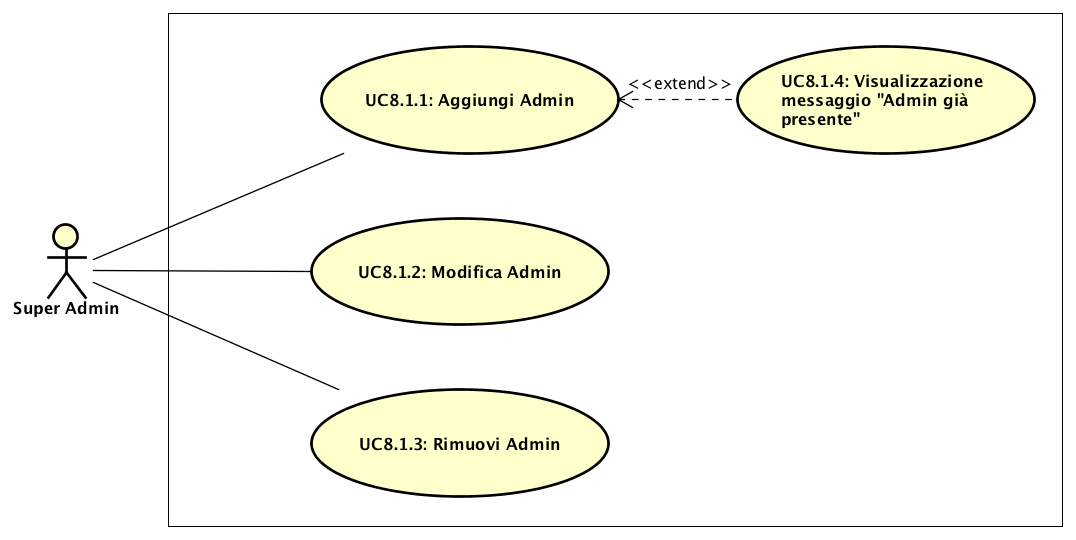
\includegraphics[width=\textwidth]{UseCases/UC8_GestionePannelloSuperadmin/UC8_1_GestioneAmministratori/UC8_1_GestioneAmministratori.png}
	\caption{UC8.1 - Gestione Amministratori}
\end{figure}
\begin{itemize} 
\item \textbf{Attori}: SuperAdmin.
\item \textbf{Descrizione}: il SuperAdmin può gestire tutti gli altri amministratori registrati nel sistema;
\item \textbf{Precondizione}: l'utente amministratore è correttamente loggato come SuperAdmin nel sistema e vuole gestire gli amministratori;
\item \textbf{Postcondizione}: l'utente SuperAdmin è riuscito a gestire correttamente gli amministratori presenti nel sistema;
\item \textbf{Scenario principale}: \begin{enumerate}\item Aggiungi Admin (UC8.1.1);\item Modifica Admin (UC8.1.2);\item Modifica email (UC8.1.2.1);\item Modifica password (UC8.1.2.2);\item Rimuovi Admin (UC8.1.3);\item Visualizzazione messaggio "Admin già presente" (UC8.1.4). 
 \end{enumerate}
\end{itemize} 
\subsection{UC8.1.1 - Aggiungi Admin} 
\label{sssec:UC8.1.1} 
\begin{itemize} 
\item \textbf{Attori}: SuperAdmin.
\item \textbf{Descrizione}: il SuperAdmin può registrare un nuovo amministratore nel sistema;
\item \textbf{Precondizione}: l'utente SuperAdmin vuole aggiungere un nuovo amministratore;
\item \textbf{Postcondizione}: l'utente SuperAdmin ha correttamente  aggiunto un nuovo amministratore;
\item \textbf{Scenario principale}: il SuperAdmin registra un nuovo amministratore nel sistema;
\end{itemize} 
\subsection{UC8.1.2 - Modifica Admin} 
\label{sssec:UC8.1.2} 
\begin{itemize} 
\item \textbf{Attori}: SuperAdmin.
\item \textbf{Descrizione}: il SuperAdmin può modificare i dati di un amministratore nel sistema;
\item \textbf{Precondizione}: l'utente SuperAdmin vuole modificare i dati di un amministratore;
\item \textbf{Postcondizione}: l'utente SuperAdmin ha correttamente  modificato i dati di un amministratore;
\item \textbf{Scenario principale}: il SuperAdmin modifica i dati di un amministratore nel sistema;
\end{itemize} 
\subsection{UC8.1.2.1 - Modifica email} 
\label{sssec:UC8.1.2.1} 
\begin{itemize} 
\item \textbf{Attori}: SuperAdmin.
\item \textbf{Descrizione}: il SuperAdmin può modificare la email di un amministratore nel sistema;
\item \textbf{Precondizione}: l'utente SuperAdmin vuole modificare la email di un amministratore;
\item \textbf{Postcondizione}: l'utente SuperAdmin ha correttamente  modificato la email di un amministratore;
\item \textbf{Scenario principale}: il SuperAdmin modifica la email di un amministratore nel sistema;
\end{itemize} 
\subsection{UC8.1.2.2 - Modifica password} 
\label{sssec:UC8.1.2.2} 
\begin{itemize} 
\item \textbf{Attori}: SuperAdmin.
\item \textbf{Descrizione}: il SuperAdmin può modificare la password di un amministratore nel sistema;
\item \textbf{Precondizione}: l'utente SuperAdmin vuole modificare la password di un amministratore;
\item \textbf{Postcondizione}: l'utente SuperAdmin ha correttamente  modificato la password di un amministratore;
\item \textbf{Scenario principale}: il SuperAdmin modifica la password di un amministratore nel sistema;
\end{itemize} 
\subsection{UC8.1.3 - Rimuovi Admin} 
\label{sssec:UC8.1.3} 
\begin{itemize} 
\item \textbf{Attori}: SuperAdmin.
\item \textbf{Descrizione}: il SuperAdmin può rimuovere un amministratore dal sistema;
\item \textbf{Precondizione}: l'utente SuperAdmin vuole rimuovere un amministratore dal sistema;
\item \textbf{Postcondizione}: l'utente SuperAdmin ha correttamente  rimosso un amministratore dal sistema;
\item \textbf{Scenario principale}: il SuperAdmin rimuove un amministratore dal sistema;

\end{itemize} 
\subsection{UC8.1.4 - Visualizzazione messaggio "Admin già presente"} 
\label{sssec:UC8.1.4} 
\begin{itemize} 
\item \textbf{Attori}: .
\item \textbf{Descrizione}: il sistema visualizza un messaggio di errore perché il SuperAdmin cerca di aggiungere un nuovo Admin con email già esistente al sistema;
\item \textbf{Precondizione}: il SuperAdmin ha confermato di voler inserire un nuovo Admin al sistema;
\item \textbf{Postcondizione}: il sistema visualizza un messaggio di errore per email Admin già presente, consentendo al SuperAdmin di poter correggere le informazioni inserite;
\item \textbf{Scenario principale}: il SuperAdmin riceve un messaggio d'errore dal sistema poiché ha cercato aggiungere un nuovo Admin con email già esistente al sistema;
\end{itemize} 
\subsection{UC9 - Visualizzazione messaggio "Slack non raggiungibile"} 
\label{sssec:UC9} 
\begin{itemize} 
\item \textbf{Attori}: Admin, Ospite, SuperAdmin.
\item \textbf{Descrizione}: Slack non è raggiungibile e viene quindi visualizzato all'utente o all'ospite il relativo messaggio di errore;
\item \textbf{Precondizione}: il sistema ha elaborato la risposta di un utente o ospite tramite Alexa e la inoltra ad Slack;
\item \textbf{Postcondizione}: il sistema visualizza un messaggio di errore perché Slack non è raggiungibile, non riuscendo quindi ad inviare il messaggio;
\item \textbf{Scenario principale}: Slack non è raggiungibile e l'utente o l'ospite ricevono dal sistema il relativo messaggio di errore;
\end{itemize} 
\subsection{UC10 - Visualizzazione messaggio "Alexa non ha compreso"} 
\label{sssec:UC10} 
\begin{itemize} 
\item \textbf{Attori}: Ospite.
\item \textbf{Descrizione}: Alexa non è stato in grado di elaborare l'input vocale ricevuto e viene quindi visualizzato all'utente o all'ospite il relativo messaggio di errore;
\item \textbf{Precondizione}: il sistema ha ricevuto risposta da un utente o ospite e la inoltra ad Alexa;
\item \textbf{Postcondizione}: il sistema visualizza un messaggio di errore perché Alexa non è riuscito ad elaborare l'input ricevuto, consentendo quindi all'utente o ospite di ripetere l'azione;
\item \textbf{Scenario principale}: Alexa non è stato in grado di elaborare l'input vocale ricevuto e l'utente o l'ospite ricevono il relativo messaggio di errore;
\end{itemize} 
\subsection{UC11 - Visualizzazione messaggio "Alexa non raggiungibile"} 
\label{sssec:UC11} 
\begin{itemize} 
\item \textbf{Attori}: Ospite, Utente.
\item \textbf{Descrizione}: Alexa non è raggiungibile e viene quindi visualizzato all'utente o all'ospite il relativo messaggio di errore;
\item \textbf{Precondizione}: il sistema ha ricevuto risposta da un utente o ospite e la inoltra ad Alexa;
\item \textbf{Postcondizione}: il sistema visualizza un messaggio di errore perché Alexa non è raggiungibile, non riuscendo quindi a comprendere l'input ricevuto;
\item \textbf{Scenario principale}: Alexa non è raggiungibile e l'utente o l'ospite ricevono il relativo messaggio di errore;
\end{itemize} 

\end{document}
